\documentclass{standalone}
\usepackage{tikz}
\usepackage{pgfplots}
\pgfplotsset{width=32cm,height=18cm,compat=1.3}
\pgfplotsset{every tick label/.append style={font=\Huge}}
\usepackage{filecontents}

\usetikzlibrary{patterns}

\definecolor{citrine}{rgb}{0.89, 0.82, 0.04}

\begin{document}
	\centering
		\vspace{1.5em}
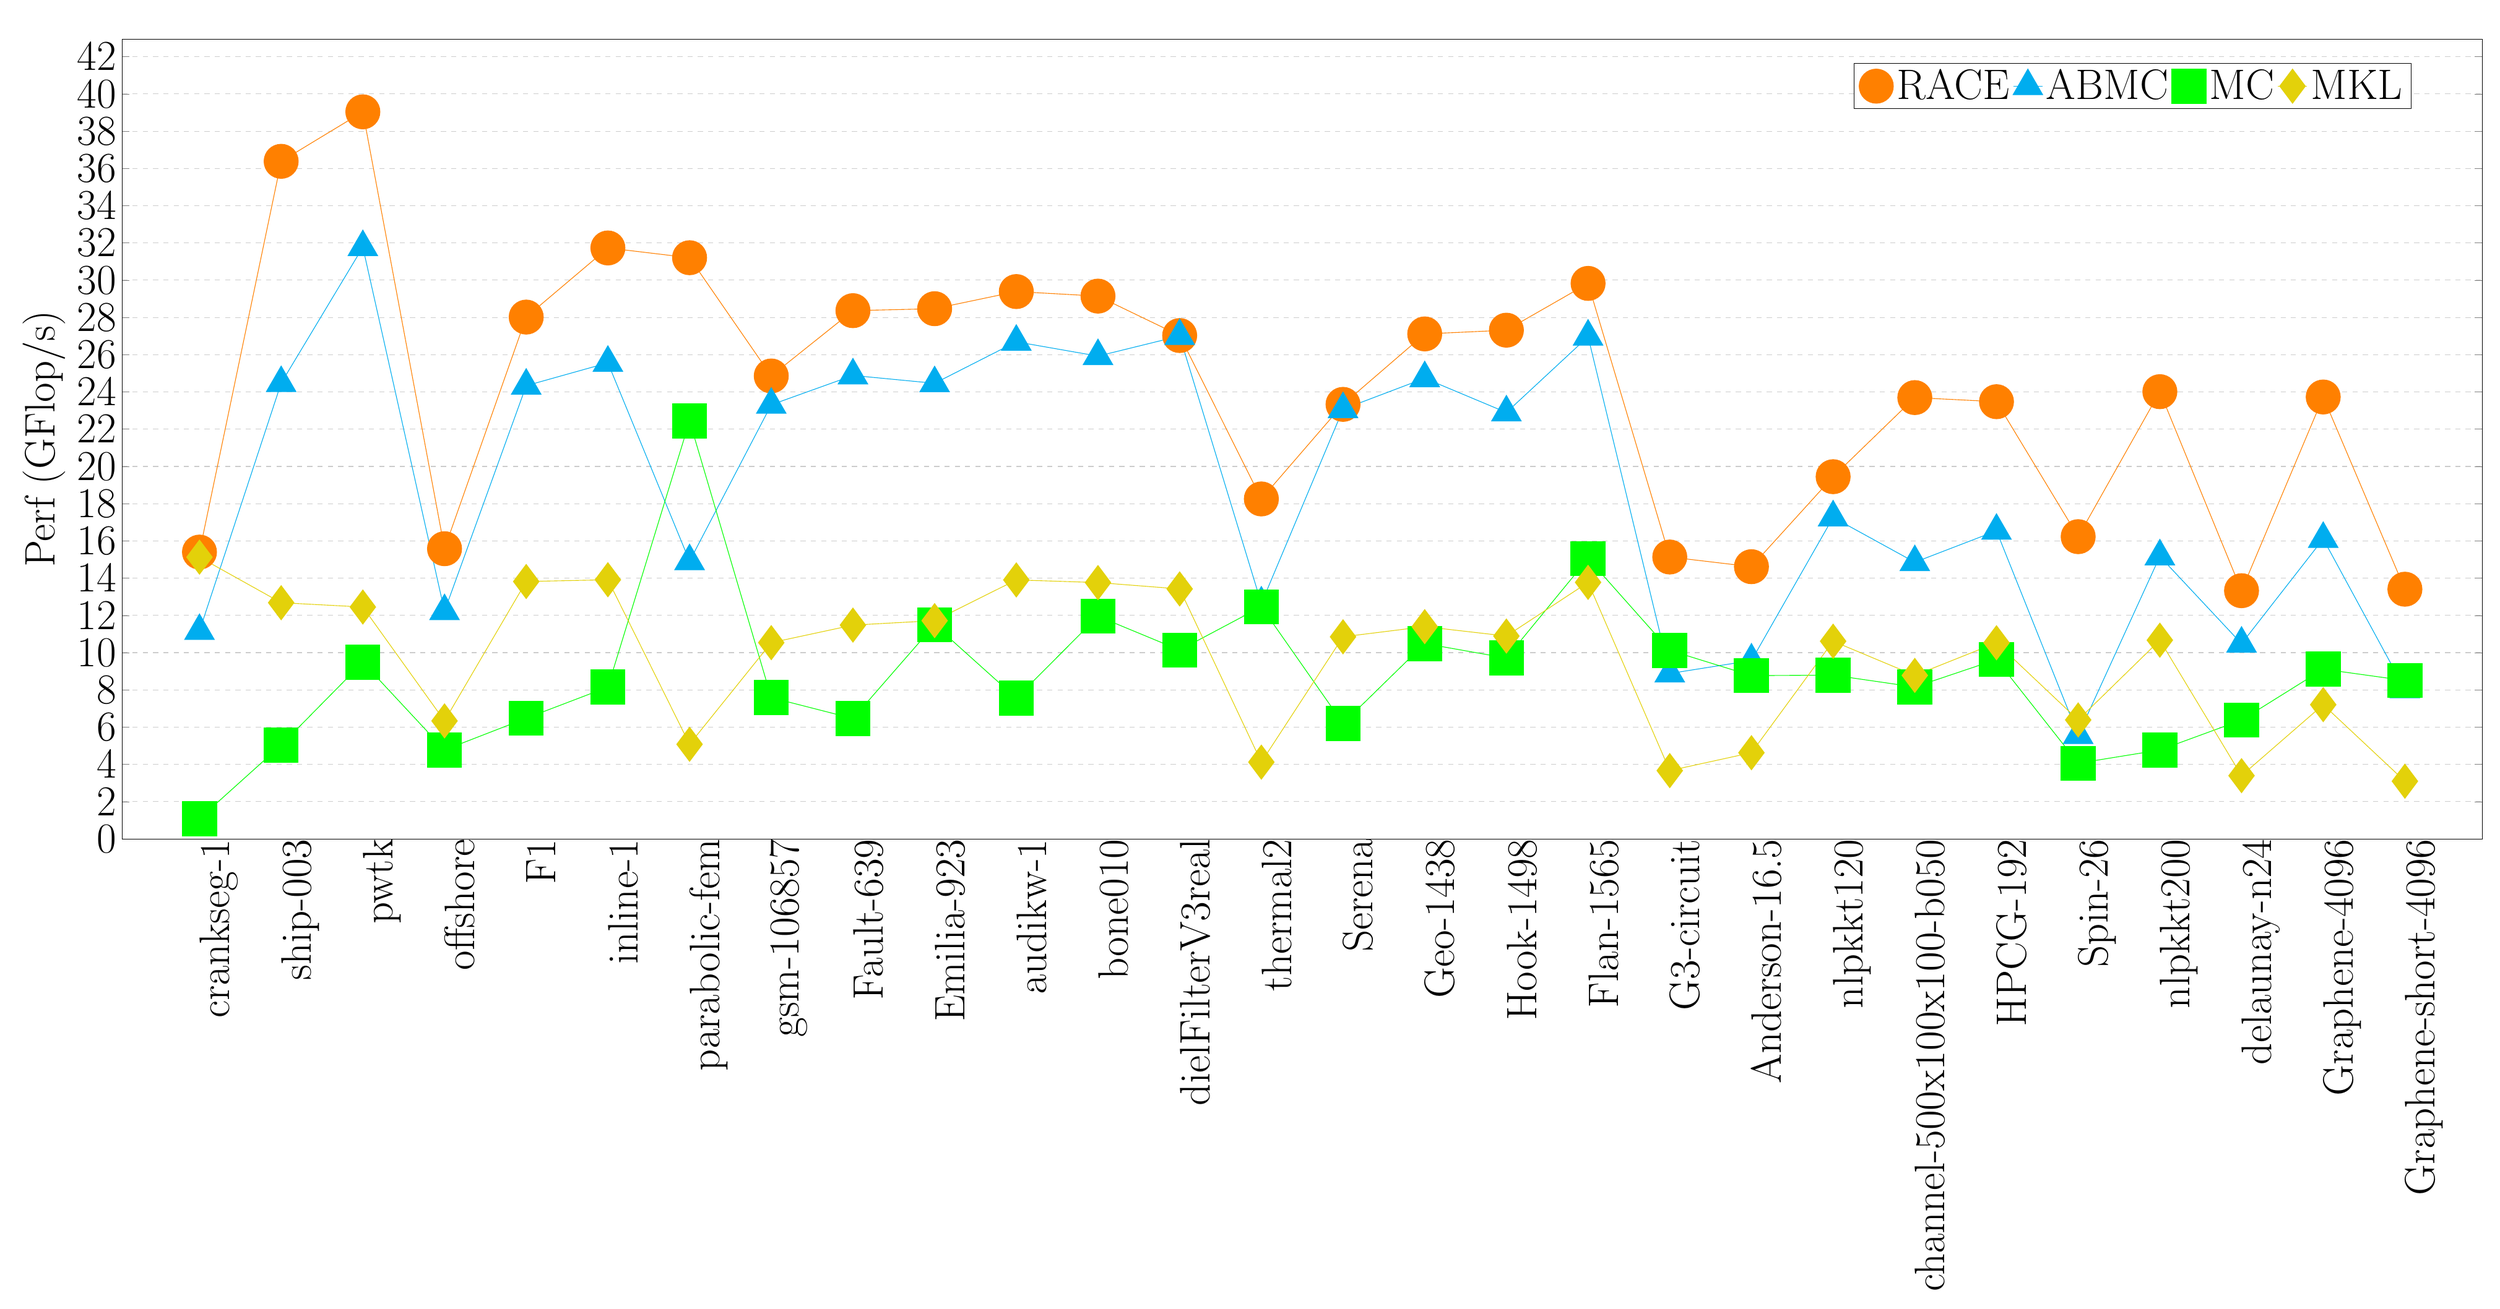
\begin{tikzpicture}
		%	\node at (13.25,15) {\LARGE{}};
			\begin{axis}[
		%	xmin=0.25, xmax=7.25,
			ymin=0, %ymax=3.25,
			xtick={1, 2, 3, 4, 5, 6, 7, 8, 9, 10, 11, 12, 13, 14, 15, 16, 17, 18, 19, 20, 21, 22, 23, 24, 25, 26, 27, 28},
		%	ytick={0,0.5,1,1.5,2,2.5,3},
			xticklabels={crankseg-1, ship-003, pwtk, offshore, F1, inline-1, parabolic-fem, gsm-106857, Fault-639, Emilia-923, audikw-1, bone010, dielFilterV3real, thermal2, Serena, Geo-1438, Hook-1498, Flan-1565, G3-circuit, Anderson-16.5, nlpkkt120, channel-500x100x100-b050, HPCG-192, Spin-26, nlpkkt200, delaunay-n24, Graphene-4096, Graphene-short-4096},
			width  = 50cm,
			height = 18cm,
			major x tick style = transparent,
			%	minor ytick={1, 5, 10, 15, 20, 25, 30 ,35,40},
			grid = minor,	
			%add_bar_commands
			ymajorgrids = true,
			grid style={dashed, gray!40},
			ylabel = {\Huge{Perf (GFlop/s)}},
		%	symbolic x coords={Graphene-2048-2048, Graphene-4096-4096, Spin-24-24-24},
			x tick label style={rotate=90, anchor=north east, inner sep=0mm, font={\Huge}},
			tick label style={font={\Huge}},
			scaled y ticks = false,
			enlarge x limits=0.035,
			legend cell align=left,
			legend style={font=\Huge},
			legend columns=-1,
			legend style={
				%at={(1,1.05)},
				%anchor=south east,
				%column sep=1ex,
				legend pos=north east
			},
			%spl_legend_code
			title= {\Huge\scalebox{1.5}{{}}}
			]

\addplot[ mark=*, mark size=10pt, mark options={orange}, draw=orange ] plot coordinates{(1,15.400558) (2,36.382835) (3,39.039620) (4,15.581563) (5,28.019140) (6,31.731108) (7,31.206720) (8,24.857203) (9,28.363801) (10,28.469068) (11,29.389081) (12,29.144620) (13,27.028246) (14,18.254121) (15,23.331850) (16,27.115273) (17,27.315481) (18,29.827848) (19,15.135629) (20,14.616334) (21,19.448762) (22,23.696725) (23,23.475947) (24,16.228225) (25,24.014094) (26,13.326586) (27,23.728702) (28,13.406762)};
\addplot[ mark=triangle*, mark size=10pt, mark options={cyan}, draw=cyan ] plot coordinates{(1,11.163256) (2,24.473980) (3,31.773709) (4,12.226397) (5,24.335161) (6,25.563684) (7,14.909928) (8,23.309563) (9,24.884935) (10,24.463317) (11,26.691912) (12,25.922877) (13,27.002845) (14,12.637824) (15,23.071445) (16,24.735392) (17,22.896719) (18,26.968986) (19,8.881203) (20,9.576315) (21,17.262901) (22,14.855593) (23,16.542055) (24,5.575682) (25,15.168208) (26,10.481901) (27,16.107057) (28,8.030951)};
\addplot[ mark=square*, mark size=10pt, mark options={green}, draw=green ] plot coordinates{(1,1.089260) (2,5.035905) (3,9.485422) (4,4.775228) (5,6.477445) (6,8.152250) (7,22.442706) (8,7.586484) (9,6.463805) (10,11.497219) (11,7.557220) (12,11.955643) (13,10.138863) (14,12.467748) (15,6.198454) (16,10.488210) (17,9.710800) (18,15.055210) (19,10.123796) (20,8.766058) (21,8.792019) (22,8.154977) (23,9.630983) (24,4.061799) (25,4.772032) (26,6.379342) (27,9.115191) (28,8.504333)};
\addplot[ mark=diamond*, mark size=10pt, mark options={citrine}, draw=citrine ] plot coordinates{(1,15.128045) (2,12.681565) (3,12.450624) (4,6.335282) (5,13.819463) (6,13.914751) (7,5.080762) (8,10.536596) (9,11.479111) (10,11.719024) (11,13.905950) (12,13.762963) (13,13.421768) (14,4.121771) (15,10.850879) (16,11.396222) (17,10.891869) (18,13.774962) (19,3.666125) (20,4.627374) (21,10.614482) (22,8.778970) (23,10.531267) (24,6.386799) (25,10.669808) (26,3.394898) (27,7.207217) (28,3.096705)};
	%addplot cmd

	\legend{RACE, ABMC, MC, MKL}

	\end{axis}			
\end{tikzpicture}

\end{document}

